\documentclass{article}

\usepackage[english]{babel}
\usepackage[utf8]{inputenc}
\usepackage{fancyhdr}
\usepackage{amsmath}

\usepackage[a4paper, total={7in, 10in}]{geometry}
\usepackage{graphicx}

\graphicspath{ {./images/} }

\pagestyle{fancy}
\fancyhf{}
\fancyhead[L]{\leftmark}
\fancyhead[R]{\thepage}

% New commands
    \newcommand{\vect}[1]{\left[\begin{array}{c}#1\end{array}\right]}
    \newcommand{\ifcases}[1]{\left\{\begin{array}{cc}\end{array}\right.}
% 

\title{SyArm Mechanics}
\author{Samuel Nösslböck}
\date{April 2022}

\begin{document}

\maketitle

\section{Introduction}
    This article is all about the mechanics of the SyArm. It is important to know which forces the load applies on which parts of the robot.
    
\section{Servo replacement}
    As servo motors do not have enough torque to withstand the forces created by the load and the arms own weight, they have to be replaced by electronic cylinders. But as cylinders can only extend and descend they need to be build in between the joints, which requires additional vector mathematics to convert the angle previously needed for the servo motors into an extension for the cylinders.
    
    \begin{center}
        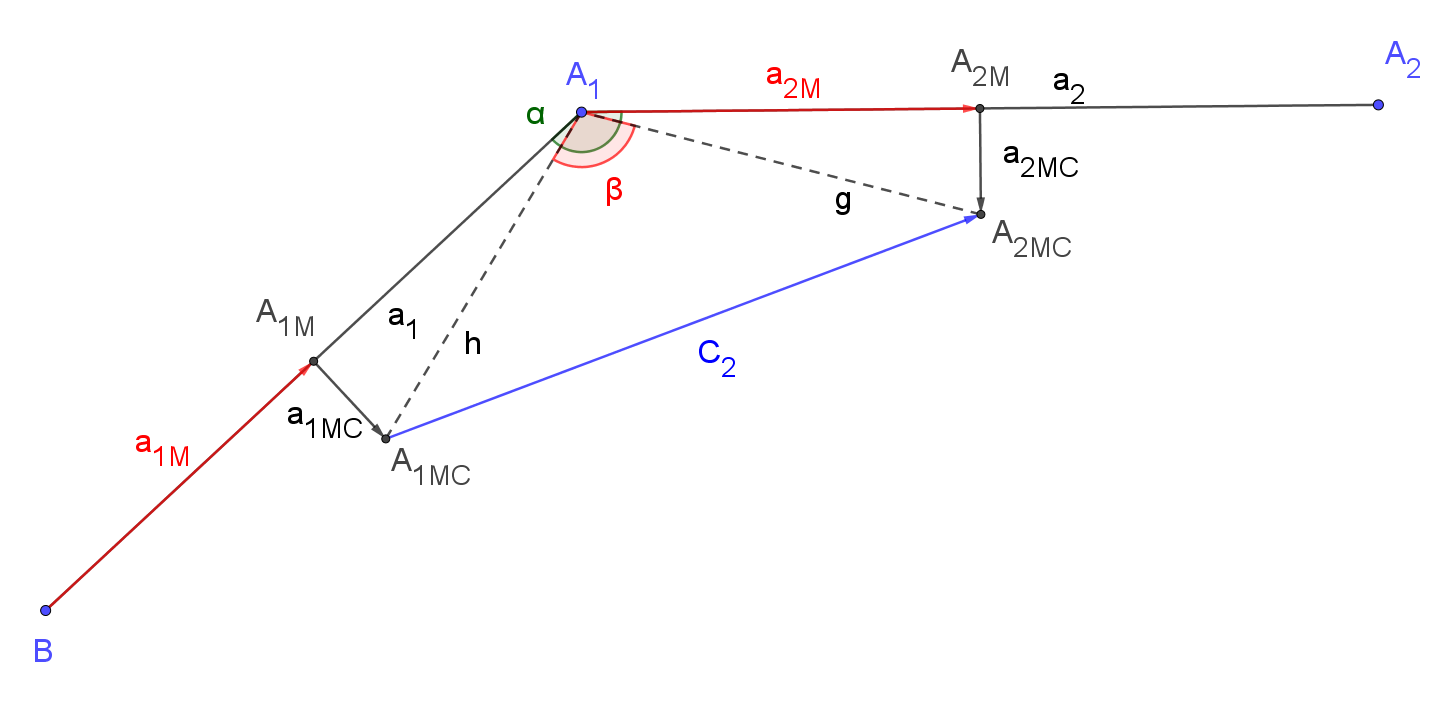
\includegraphics[scale=0.45]{images/Cylinder.PNG}
    \end{center}
    
    The schematic above shows the second cylinder $C_2$, which is responsible for the angle in joint $A_2$. However the following equations can be applied to every cylinder when using the corresponding lengths instead of the ones used in this overall definition.
    
    As many of the vectors are representing the construction their length is therefore known and can be used as constants:
    
    \begin{equation}
        |\vec{a_{1}}| = \text{const} \quad |\vec{a_{2}}| = \text{const} \quad |\vec{a_{1M}}| = \text{const} \quad |\vec{a_{2M}}| = \text{const} \quad |\vec{a_{1MC}}| = \text{const} \quad |\vec{a_{1MC}}| = \text{const}
    \end{equation}
    
    The control script now gets a position and calculates the angle $\alpha$. When knowing this angle, the script can calculate the length of the cylinder $C_2$ needed to match the angle.
    
    \begin{equation}
        h = \sqrt{ |\vec a_1 - \vec a_{1M}|^2  + {\vec{a_{1MC}}}^2 } \quad g = \sqrt{ | \vec a_2 - \vec a_{2M}|^2  + {\vec{a_{2MC}}}^2 }
    \end{equation}
    
    \begin{equation}
        \beta = \alpha - \arcsin{ \left(\frac{|\vec{a_{2MC}}|}{g}\right) } - \arcsin{ \left(\frac{|\vec{a_{1MC}}|}{h}\right) }
    \end{equation}
    
    Applying the law of cosines, $C_2$ can be calculated with
    
    \begin{equation}
        \begin{array}{c}
            {C_2}^2 = g^2 + h^2 - 2gh\cos(\beta) 
        \end{array}
    \end{equation}
    
    When knowing the minimum and maximum length of the cylinder $C_{min}$ and $C_{max}$, the minimum and maximum angle of $\beta$ can be calculated using
    
    \begin{equation}
        \beta_{min/max} = \arccos{ \left( \frac{a^2 + b^2 - {C_{min/max}}^2}{2ab} \right ) }
    \end{equation}
    
\section{Angular speed of cylinders}
    The cylinders used to replace the servo motors have a given extension speed $v_C$ which means their total cylinder length results in the integral of this constant.
    
    \begin{equation}
        C(t) = \int v_C dt = v_C t + C_0
    \end{equation}
    
    When using the formula for section two for the inner angle $\beta$ and inserting the equation above for the dependency in cylinder length, the formula now gets a dependency of time.
    
    \begin{equation}
        \beta(C(t)) = \arccos{ \left( \frac{a^2 + b^2 - C(t)^2}{2ab} \right ) } \xrightarrow{} 
        \beta(t) = \arccos{ \left( \frac{a^2 + b^2 - v_C^2t^2 - 2 v_C t C_0 - C_0^2}{2ab} \right ) }
    \end{equation}
    
    Now that $\beta$ has its dependency over time, the angular speed can be calculated using the derivative of the equation above.
    
    \begin{equation}
        \omega(t) = \frac{d\beta}{dt} = \frac{2 C(t)}{\sqrt{- C(t)^4 - g^4 - h^4 + 2c^2 + g^2 + h^2 + 2 g^2 h^2}}
    \end{equation}

\section{Optimizing angle span}
    As the SyArm should be able to reach as much space as easy as possible, the concept of the angle span is important. 
    
    \begin{equation}
        \beta_{span} = \beta_{max} - \beta_{min}
    \end{equation}
    
\section{Cylinder forces}
    To clarify the calculation of all forces and loads acting on the arm, each part is treated separately. However a few formulas can be generally defined, as they are true for all cylinder cases.
    
    The following equations are all based on the fundamental principal of statics
    
    \begin{equation}
        \sum \vec{M_n} = 0 \quad \sum \vec{F_n} = 0
    \end{equation}
    
    The force acting on every cylinder balances the torque in the given arm section
    
    \begin{equation}
        \vec F_{Cn}  = \frac{|\sum \vec M_{A n - 1} |}{| \vec C_n \times \vec a_n |} \cdot \vec C_n
    \end{equation}
    
    and the force acting on the joint in this section balances all acting forces
    
    \begin{equation}
        \vec{F_{An - 1}} = - \sum \vec F_n
    \end{equation}
    
    \textbf{First Section}
    
        \begin{center}
            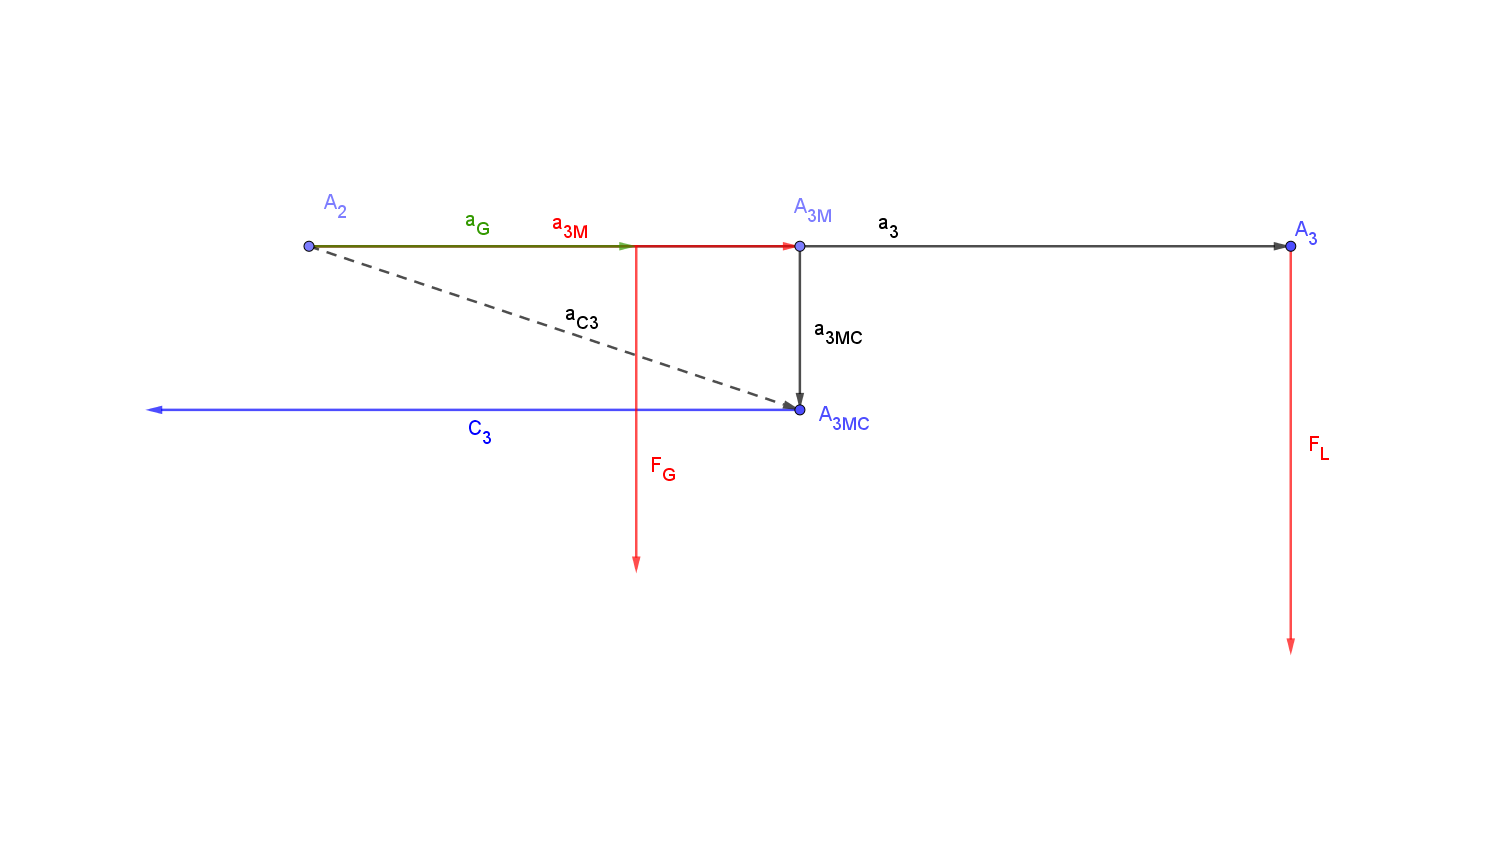
\includegraphics[scale=0.5]{images/Section3.PNG}
        \end{center}
        
        \begin{equation}
            m_L = \text{const} \quad m_{G3} = \text{const} \quad |\vec{a_3}| = \text{const}
        \end{equation}
        
        \begin{equation}
            \vec F_L = \vect{ 0 \\ 0 \\ m_L g} \quad \vec F_{G3} = \vect{ 0 \\ 0 \\ m_{G3} g} \quad \vec a_{C3} = \vec a_{3M} + \vec a_{3MC}
        \end{equation}
        
        \begin{equation}
            \vec F_{C3} = \frac{| \vec F_L \times \vec a_3 + \vec F_{G3} \times \vec a_{G3}|}{| \vec C_3 \times \vec a_{C3} |} \cdot \vec C_3 \quad
            \vec F_{A2} = - ( \vec F_L + \vec + F_{G3} - \vec F_{C3} )
        \end{equation}
    
    \textbf{Second Section}
    
        \begin{center}
            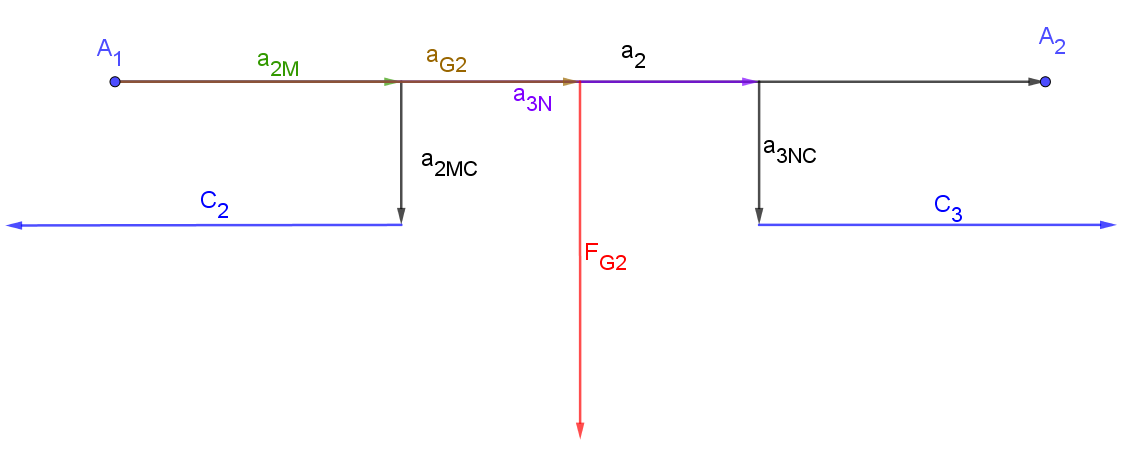
\includegraphics[scale=0.5]{images/Section2.PNG}
        \end{center}
        
        \begin{equation}
            m_L = \text{const} \quad m_{G3} = \text{const} \quad |\vec{a_3}| = \text{const}
        \end{equation}

\end{document}